\chapter{Projektbeskrivelse}

\section{Projektgennemførelse}
Projektet startede med, at der blev lavet en tidsplan, hvor der var mulighed for ændringer undervejs, dog var der nogle faste deadlines, som skulle følges. De forskellige deadlines ledte op til, at man kunne arbejde efter vandfaldsmodellen, da projektet startede med, at der blev lavet kravspecifikation og accepttest, som beskrev de krav, som programmet skulle kunne udfylde. Derefter var næste deadline, at der skulle laves design, ligesom viste forskellige diagrammer over, hvordan programmet skulle opbygges og hvad der skulle indeholde. Derefter blev programmeret færdiggjort og testet og til sidst finpudset. \\ \\
Altså er der i dette projekt blevet arbejdet efter vandfaldsmodellen, som er benyttes, man arbejder med software, ligesom der er blevet gjort i det pågældende projekt. Vandfaldsmodellen er opbygget på sådan en måde, at man arbejder med de forskellige dele som et vandfald, hvor man tager en af del afgangen og bevæger sig ned gennem de forskellige. De forskellige deadlines vi har haft stemmeroverens med de forskellige led i vandfaldsmodellen, som ses i figur(NUMMER)

\begin{figure}[H]
	\centering
	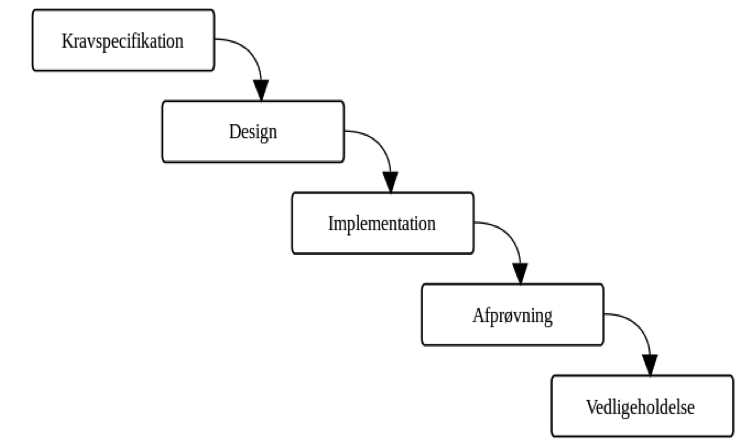
\includegraphics[width=1\textwidth]{Figurer/Snip20150522_15}
	\caption{Vandfaldsmodel}
\end{figure}

\textbf{Skal vi have blokken med vedligeholdelse med??}\\
Projektgruppen har været på 8 medlemmer, som er blevet delt ind i 2 grupper, således at arbejdsbyrden blev delt. Den ene gruppe arbejdede med softwareudviklingen, mens den anden gruppe arbejdede med dokumentation og udarbejdelsen af design. Da gruppen har været opdelt, har der været projektmøde hver uge, hvor gruppen har opdateret hinanden og rettet tidsplanen til, hvis det var nødvendigt.


\section{Metode}

\begin{itemize}
	\item Hvilke programmer, der er blevet benyttet til at besvare opgaven. Github, visual studio, LaTex, visio, googledrev, facebook. 
	\item Spørg muligvis Lars, om hvad han forventer, hvad der skal står her. 
\end{itemize}

\section{Specifikation og analyse}
SARA

\section{Arkitektur}
SARA

\subsection{Design}

\subsection{Implementering}

\section{Resultater og diskussion}

\section{Opnået erfaringer}

\section{Fremtidigt arbejde}
Som følge af at projektet er tiltænkt som en prototype, er der løbende gennem projekt udførelsen opstået en masse muligheder og ideer for videreudvikling af systemet. \\
Den første helt basale idé, som også er forsøgt udført sideløbende i projektet, er etablering af en "opret ny patient" funktion. Funktionen skal muliggøre, at den sundhedsprofessionelle kan oprette en ny patient i systemet, i forbindelse med indtastning af patientens CPR nummer. Funktionen skal fungere således, at hvis ikke det indtastede CPR nummer i forvejen er kendt i systemet, skal skridtet efter CPR-vinduet være et nyt "Opret Patient"-vindue. Her skal den sundhedsprofessionelle kunne indtaste relevante oplysninger omkring patienten, og til slut oprette patienten i både den private- og offentlige database.\\
Et ideelt område til videreudvikling er brugervenlighed, både på software plan og i særhed på hardware plan.
